\section{实验步骤}
完成本实验的主要步骤如下:
\begin{enumerate}
    \item 通过阅读官方文档学习BeautifulSoup,requests,selenium库的基本使用方法;
    \item 通过开发者工具查看网页源代码,分析中国天气网的网页结构;
    \item 通过开发者工具查看网页发送的请求,并对请求报文,回复报文进行分析;
    \item 编写Python脚本,利用上述库爬取目标数据;
    \item 存储目标数据并进行可视化。
\end{enumerate}
\subsection{获取上海市9月份数据}
图\ref{homepage}为中国天气网的主页,可以通过右上角的搜索框来跳转至各个城市对应的页面。
图\ref{shanghaihomepage},\ref{beijinghomepage}分别是上海市和北京市对应的对应的页面。
不难看出,它们的url中的“1d”代表着当前页面的显示内容为今日天气;它们url的唯一区别在于其中的一串数字,可以初步推断这是城市的代码。


\begin{figure}[!htbp]
    \centering
    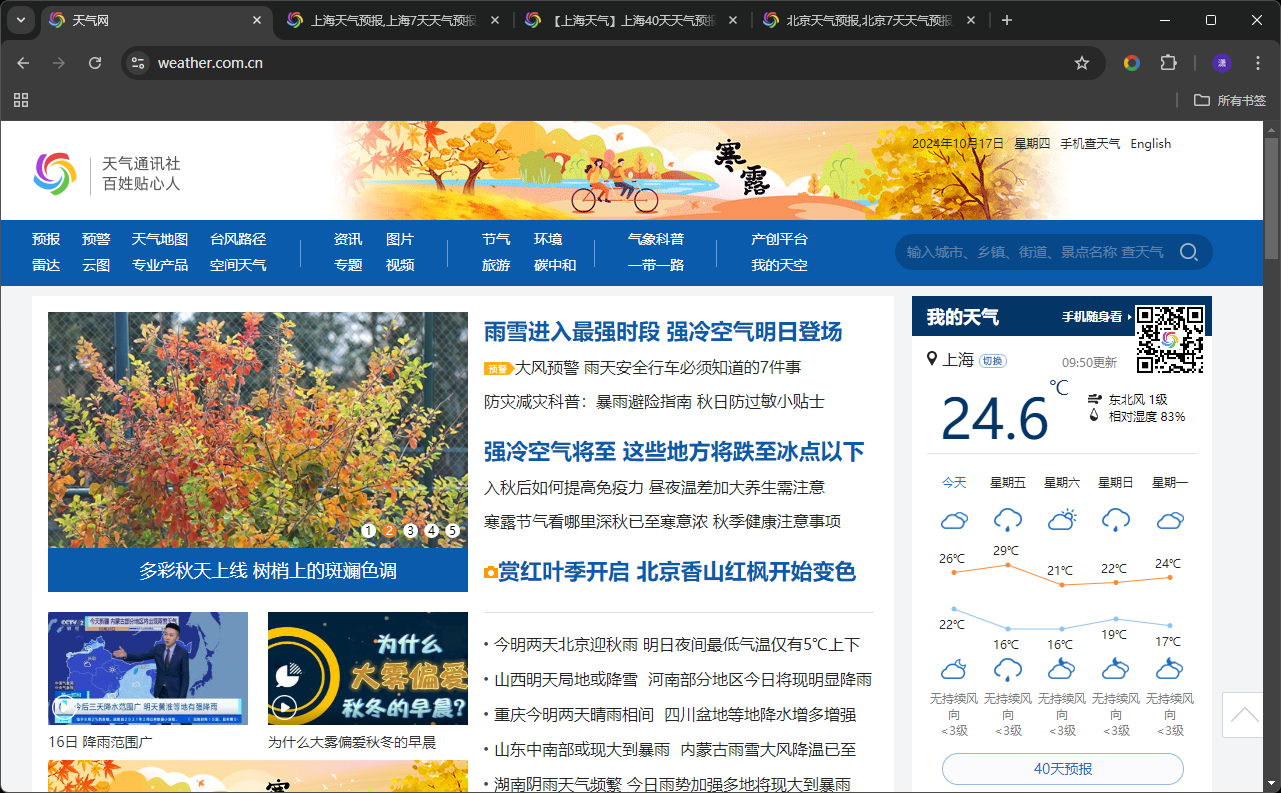
\includegraphics[width=\textwidth]{figures/homepage.png}
    \caption{中国天气网主页\url{www.weather.com.cn}}\label{homepage}
\end{figure}

\begin{figure}[!htbp]
    \centering
    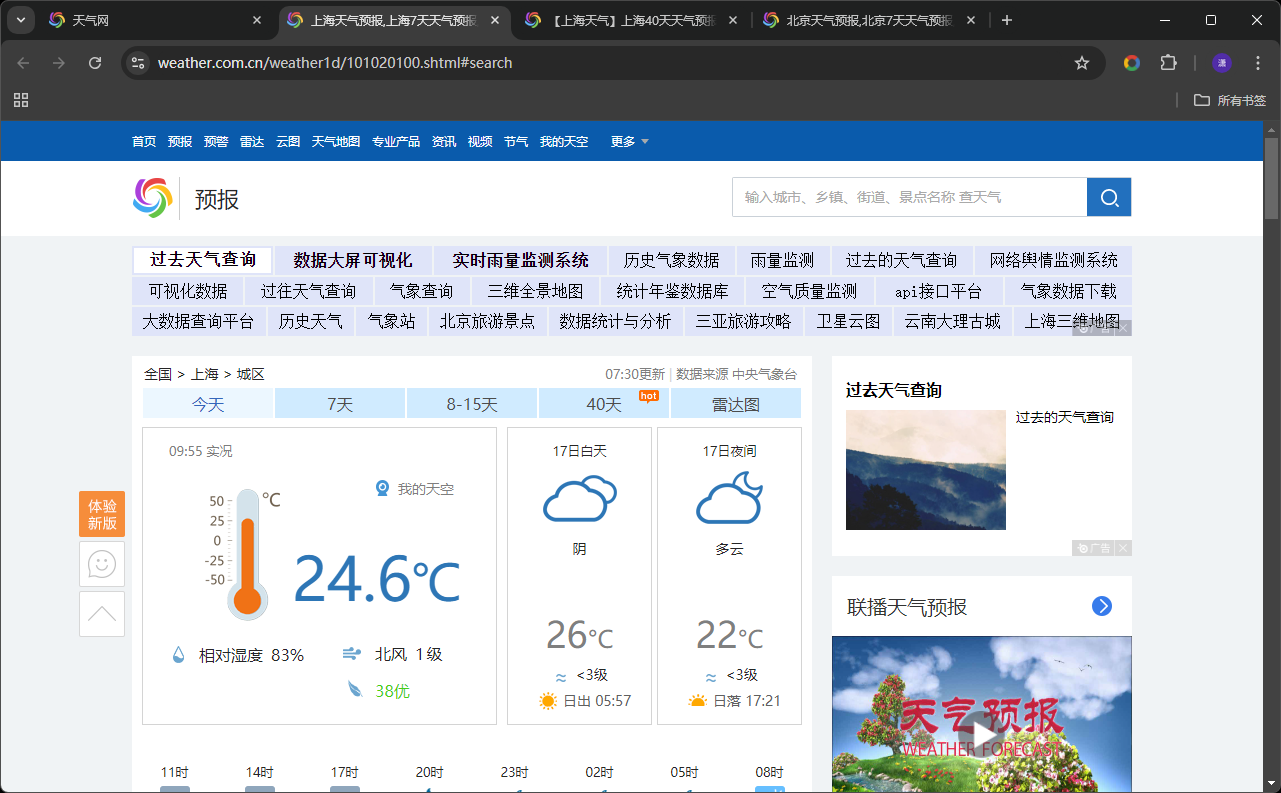
\includegraphics[width=\textwidth]{figures/shanghai_homepage.png}
    \caption{上海市天气情况页面\url{weather.com.cn/weather1d/101020100.shtml\#search}}\label{shanghaihomepage}
\end{figure}

\begin{figure}[!htbp]
    \centering
    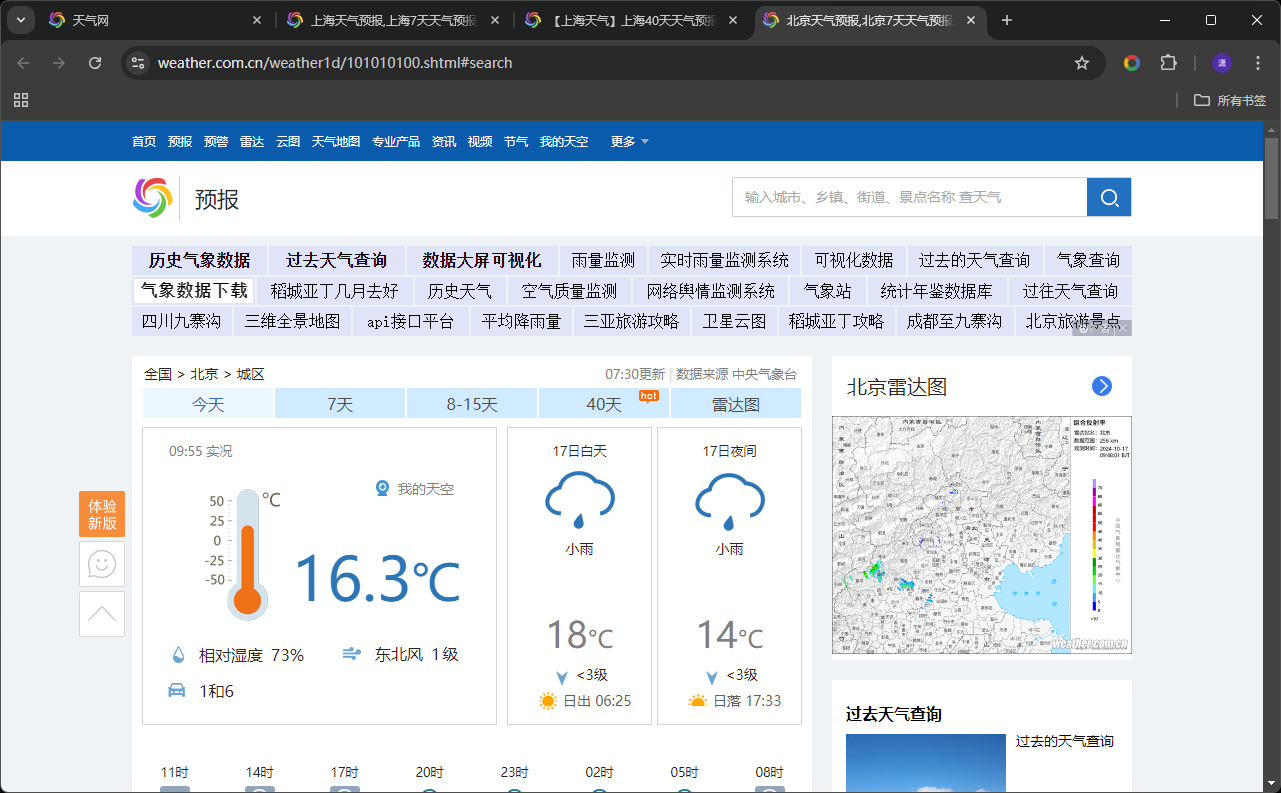
\includegraphics[width=\textwidth]{figures/beijing_homepage.png}
    \caption{北京市天气情况页面\url{weather.com.cn/weather1d/101010100.shtml\#search}}\label{beijinghomepage}
\end{figure}

点击“40天”按钮即可切换至包含40天的天气情况的日历页面,然后打开开发者工具来视察网页元素。如图\ref{inspectcalendar}所示,url中的“1d”变为了“40d”,
后跟的数字编码没有改变;本实验所需的气温信息存放在span元素中,最高气温和最低气温对应的类名分别为max和min,而span元素的父元素为类名为w\_xian的div元素,其父元素是
类名为history  的td元素,所属的表格元素的id为table。

\begin{figure}[!htbp]
    \centering
    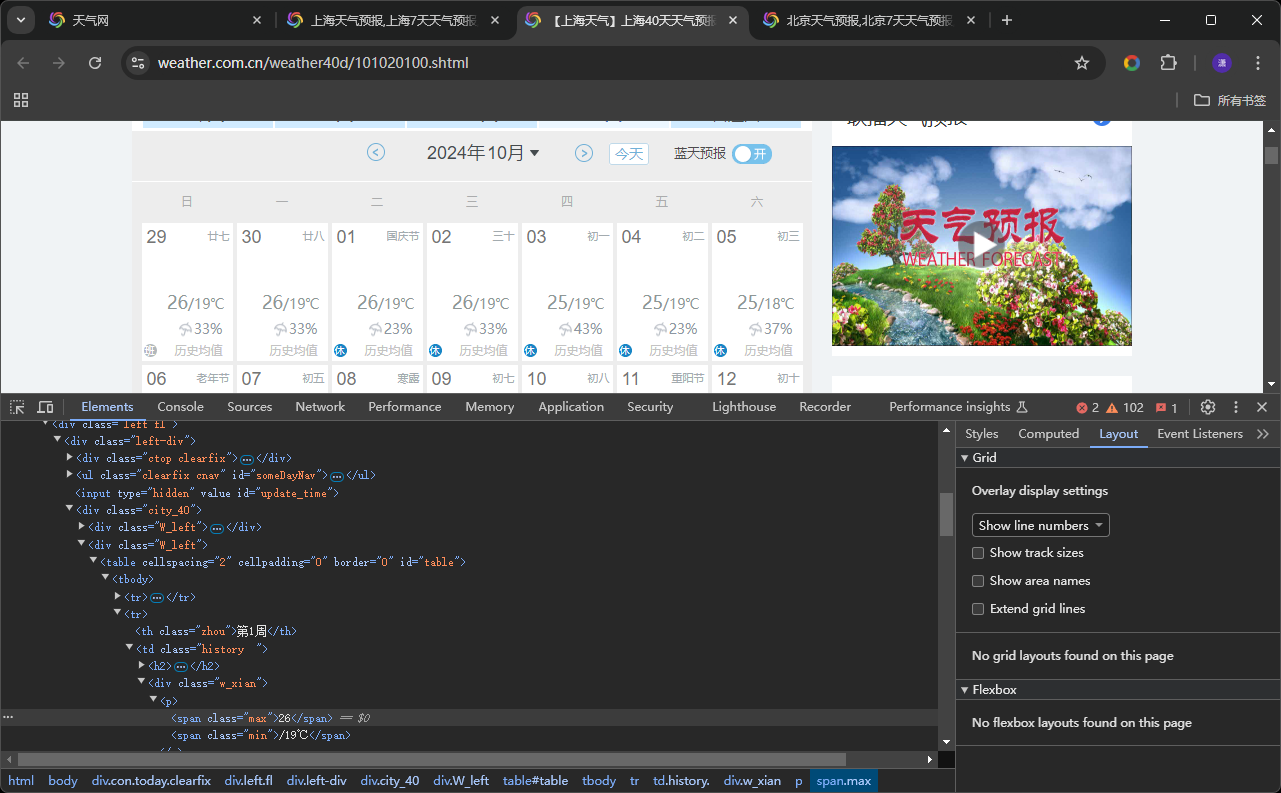
\includegraphics[width=\textwidth]{figures/inspect_calendar.png}
    \caption{存放天气信息的网页元素}\label{inspectcalendar}
\end{figure}

然后视察网络请求情况。为了观察跳转网页时发出的网络请求,如图\ref{activate}所示,我先勾选在设置中的Global大项里的Auto-open DevTools for popups选项,使得跳转页面时开发者工具栏自动打开。
接着我返回中国天气网主页,再次通过搜索栏跳转至上海市对应页面,并查看网络活动。
如图\ref{cityjs}所示,在名为city.js的请求的回复报文中,包含各个城市及其对应数字编号的信息;如图\ref{calenderresponse}所示,在另外一个请求中,
其回复报文包含了天气日历中的各类信息,图\ref{calenderheader}是该请求的请求头。该请求头的载荷只有一串数字。经过验证,该串数字为精确到毫秒的UNIX时间戳。
因此我尝试构造请求来直接获取9月的日历信息,但是如图\ref{fail}所示,并未成功获取所需的日历信息。因此,我接着尝试使用selenium来获取日历信息。

\begin{figure}[!htbp]
    \centering
    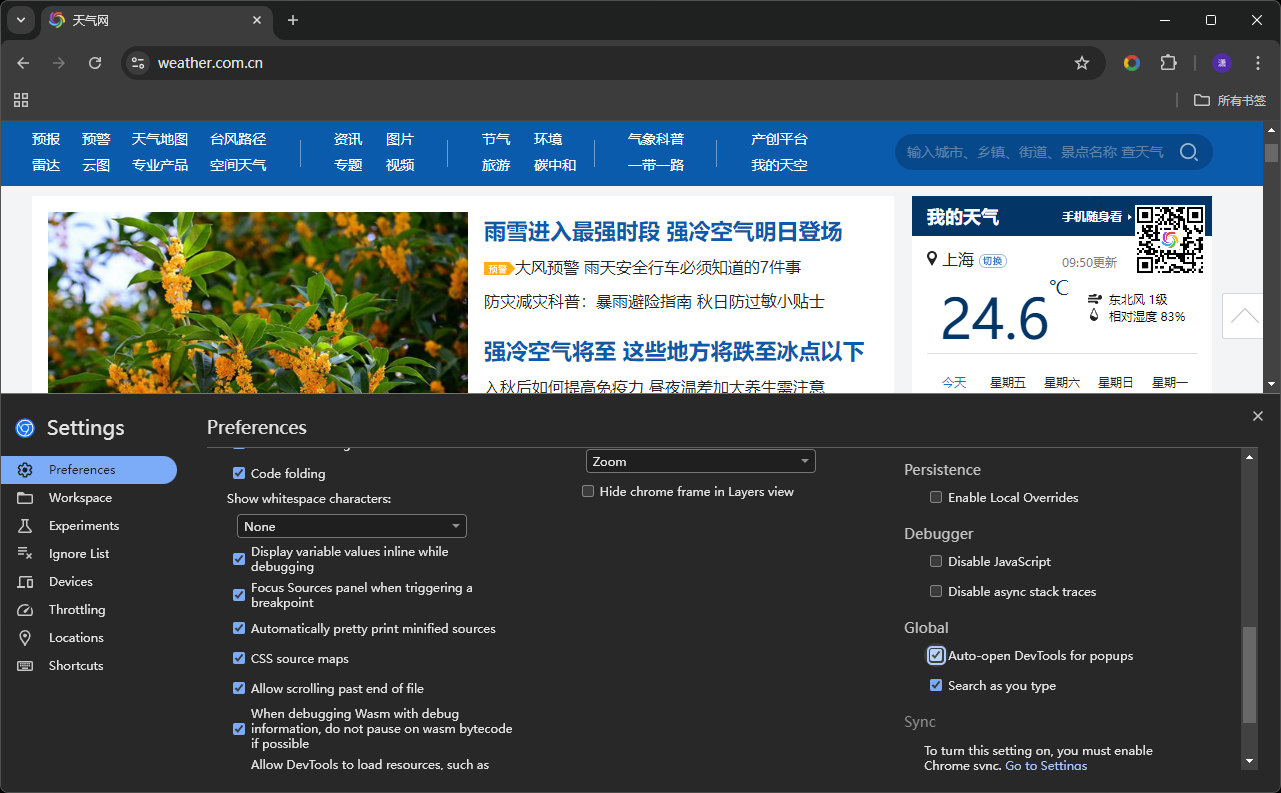
\includegraphics[width=\textwidth]{figures/activate.png}
    \caption{设置自动打开开发者工具}\label{activate}
\end{figure}

\begin{figure}[!htbp]
    \centering
    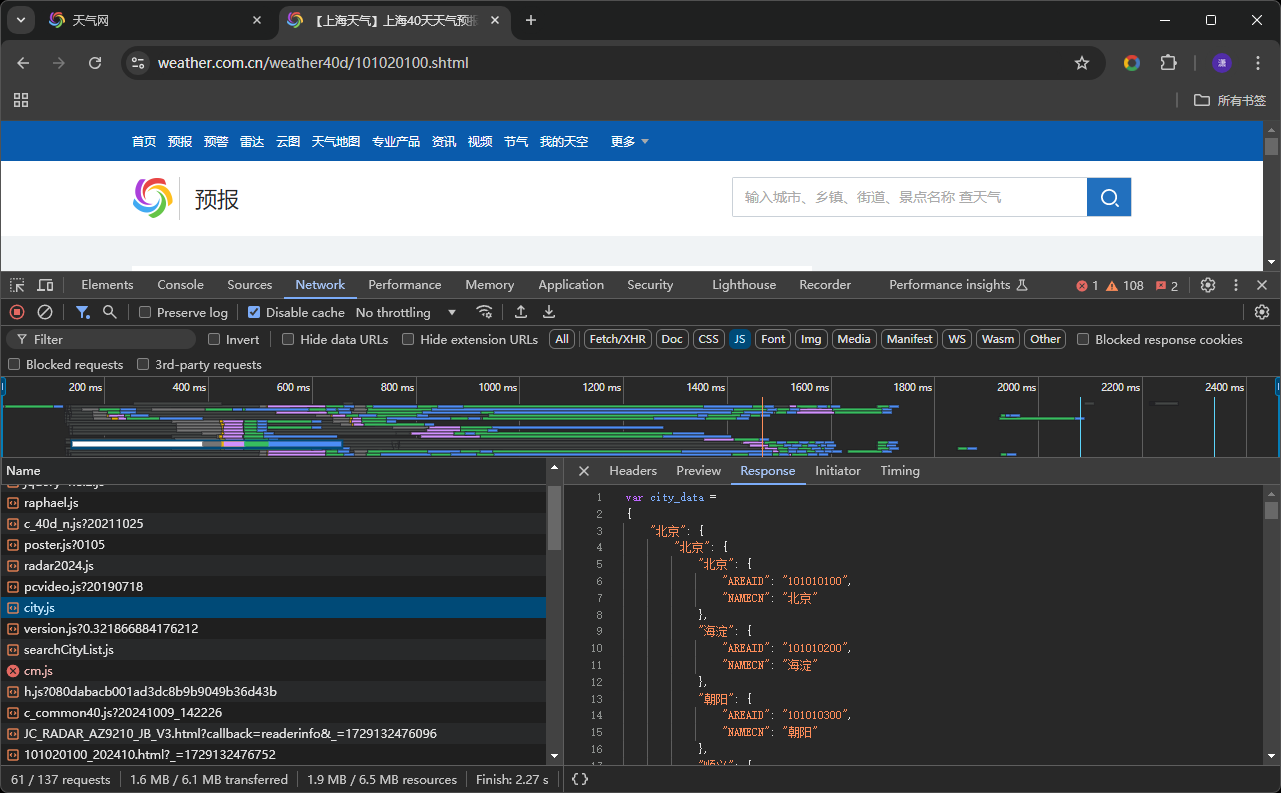
\includegraphics[width=\textwidth]{figures/city.js.png}
    \caption{含有城市编号信息的回复报文}\label{cityjs}
\end{figure}

\begin{figure}[!htbp]
    \centering
    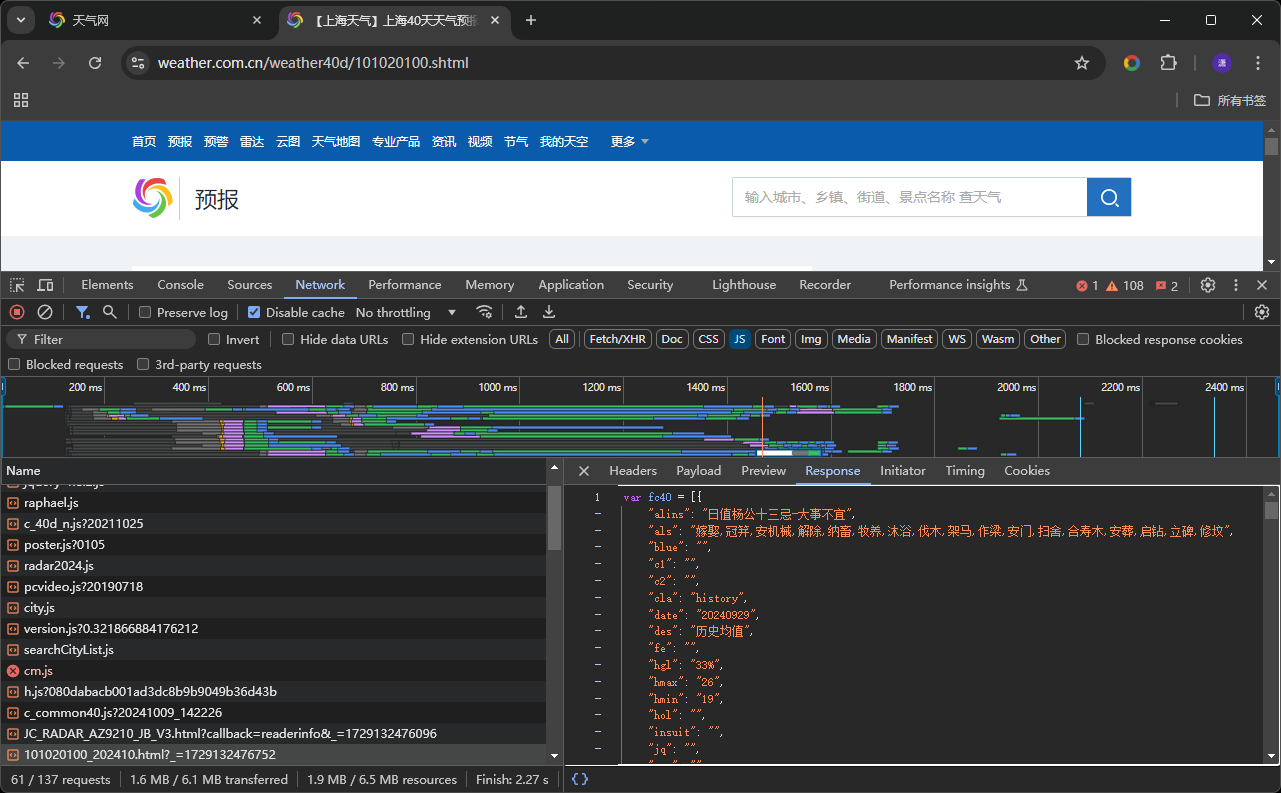
\includegraphics[width=\textwidth]{figures/calendar_response.png}
    \caption{含有气候日历信息的回复报文}\label{calenderresponse}
\end{figure}

\begin{figure}[!htbp]
    \centering
    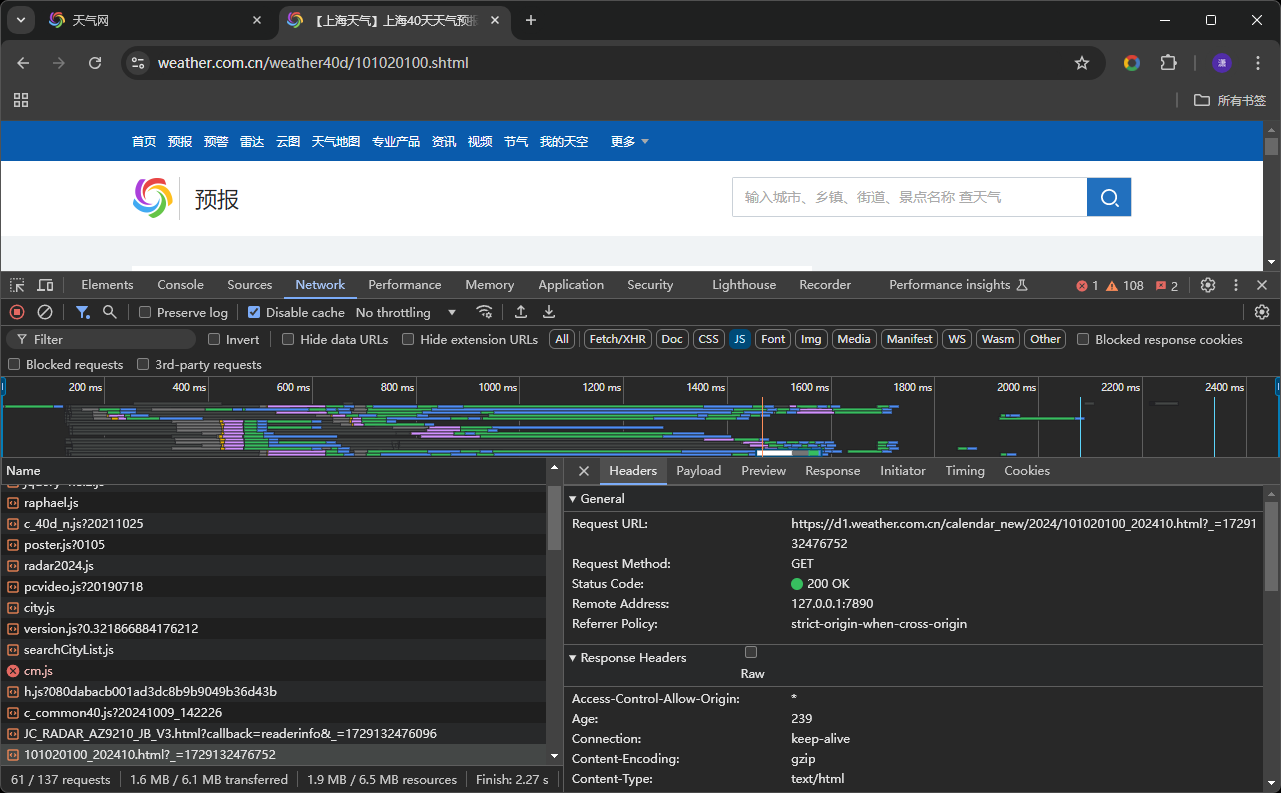
\includegraphics[width=\textwidth]{figures/calendar_header.png}
    \caption{含有气候日历信息的回复报文对应的报文头}\label{calenderheader}
\end{figure}

\begin{figure}[!htbp]
    \centering
    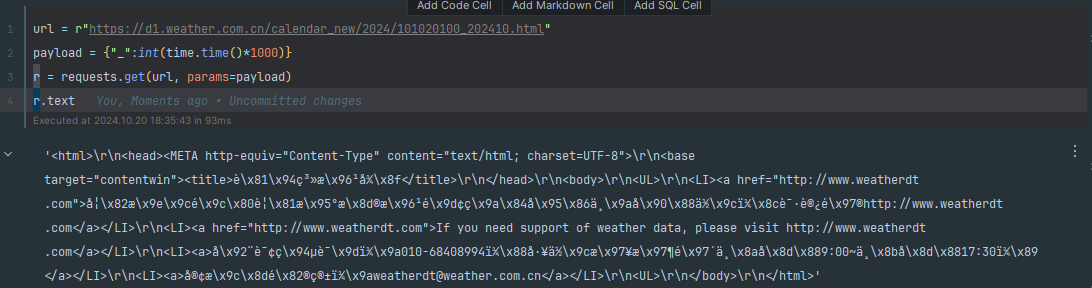
\includegraphics[width=\textwidth]{figures/fail.png}
    \caption{未成功通过请求的方式获取天气日历}\label{fail}
\end{figure}

点击按钮跳转至9月份的天气日历,如图\ref{newcalendarresponse}所示,新增请求只有一个,其回复报文内容便是日历中的信息。同时,如图\ref{locateaction}所示,我通过
控制台,我确定了触发切换页面的网页元素是类名为Y\_left的span元素。

\begin{figure}[!htbp]
    \centering
    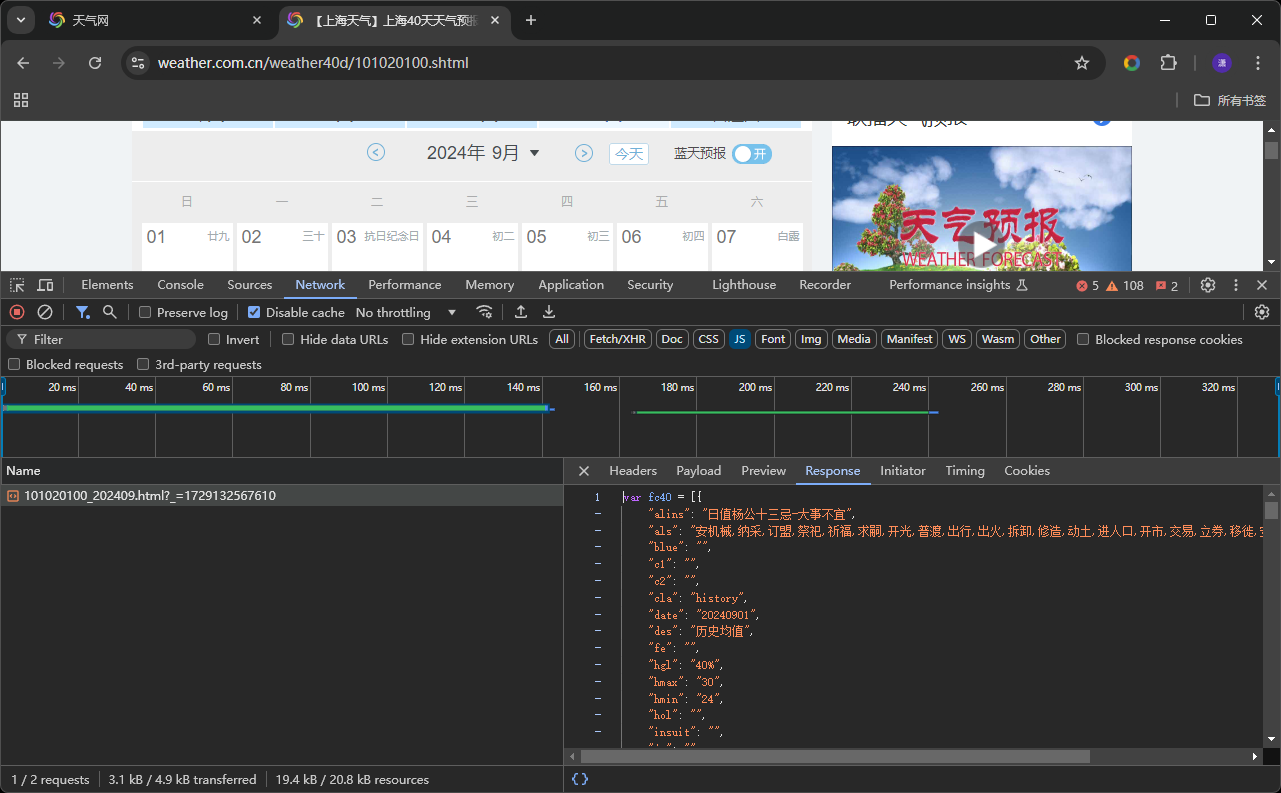
\includegraphics[width=\textwidth]{figures/new_calendar_response.png}
    \caption{切换月份时接收到的回复报文}\label{newcalendarresponse}
\end{figure}

\begin{figure}[!htbp]
    \centering
    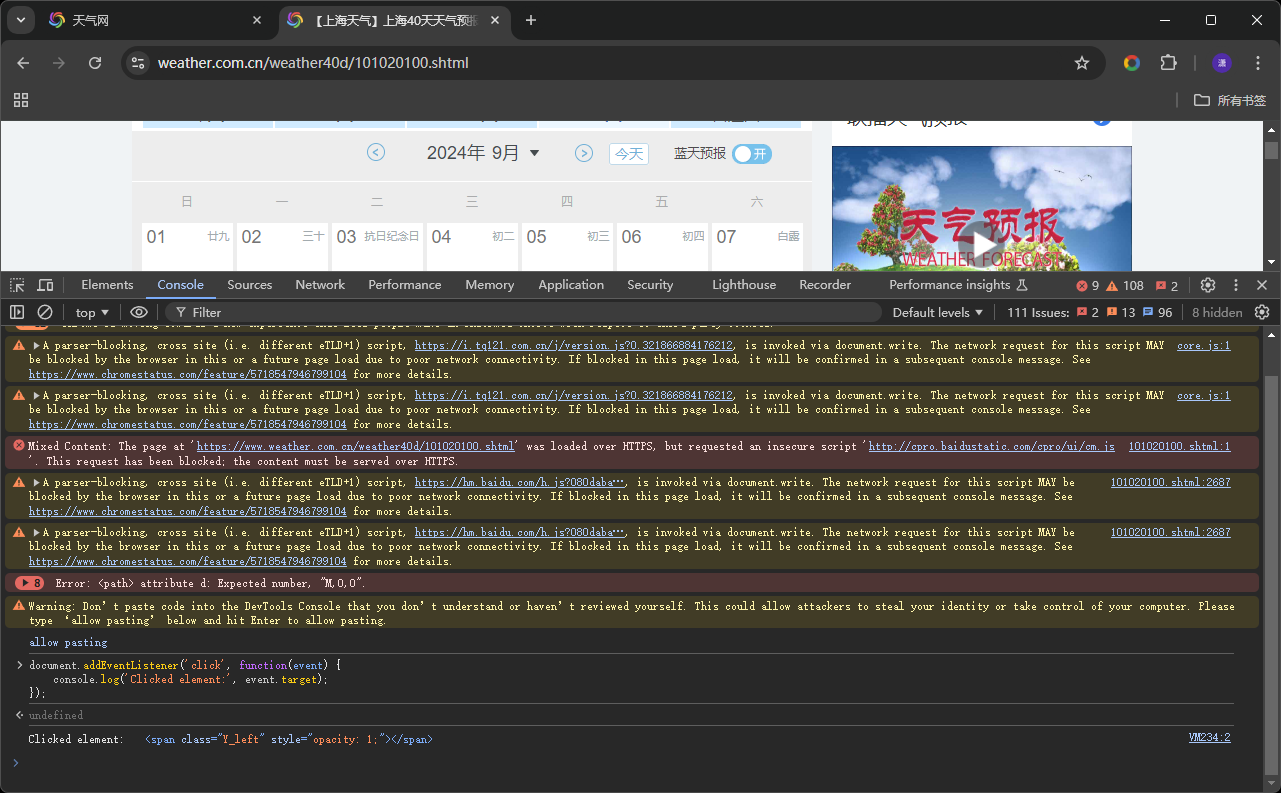
\includegraphics[width=\textwidth]{figures/locate_action.png}
    \caption{通过控制台确定触发切换月份的网页元素}\label{locateaction}
\end{figure}

综上,包含40天天气信息的网页是动态网页,同时,为了获取9月份的天气信息,需要在上海市对应页面先通过名为Y\_left的span元素切换至9月份对应页面,然后
在id为table的table元素中将天气信息提取出来。

为此,可以利用selenium库来执行切换页面的操作并获取table元素的内容,然后利用正则表达式等工具从字符串中提取气温信息。

如图\ref{success}所示,我成功使用selenium提取到了9月份上海天气日历的信息。

\begin{figure}[!htbp]
    \centering
    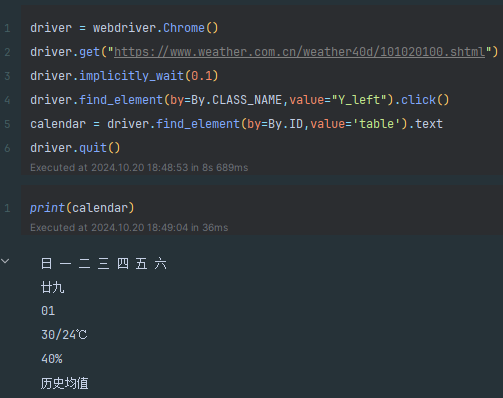
\includegraphics[scale=1]{figures/success.png}
    \caption{成功使用selenium获取日历内容}\label{success}
\end{figure}

\subsection{获取当天全国省会级城市天气信息}

点击图\ref{homepage}左上方的“天气地图”,即可加入图\ref{weathermap}所示的页面。在此页面中,点击中国地图上的位置,即可显示该处的天气信息;
也可以通过右上角的列表来选取指定城市的天气信息。

图\ref{imgboundcontent}-\ref{weatherinfoload}展示的是加载天气地图时产生的几个较为关键的网络请求的回复报文体、请求报文头、请求载荷信息。
img\_bound请求的载荷为时间戳,返回内容是各城市和地区的名称以及对应的经纬度范围;region\_list请求的载荷为时间戳,返回内容是各个城市的名称,编号以及状态;
city请求的载荷为时间戳,返回内容是各个城市的名称及其经纬度;api请求所需的载荷是经纬度坐标、方法、callback方法和时间戳,返回内容是对应的城市信息;sk请求的载荷是
经纬度坐标、callback方法和时间戳。

经过尝试,上述请求均可以通过requests库来人为构造并获取相应的回复报文。

因此,我先通过city请求来获取各城市的名称,经纬度,然后利用api和sk请求来获取各城市的信息及其气温,并存放在数据库中。

\begin{figure}[!htbp]
    \centering
    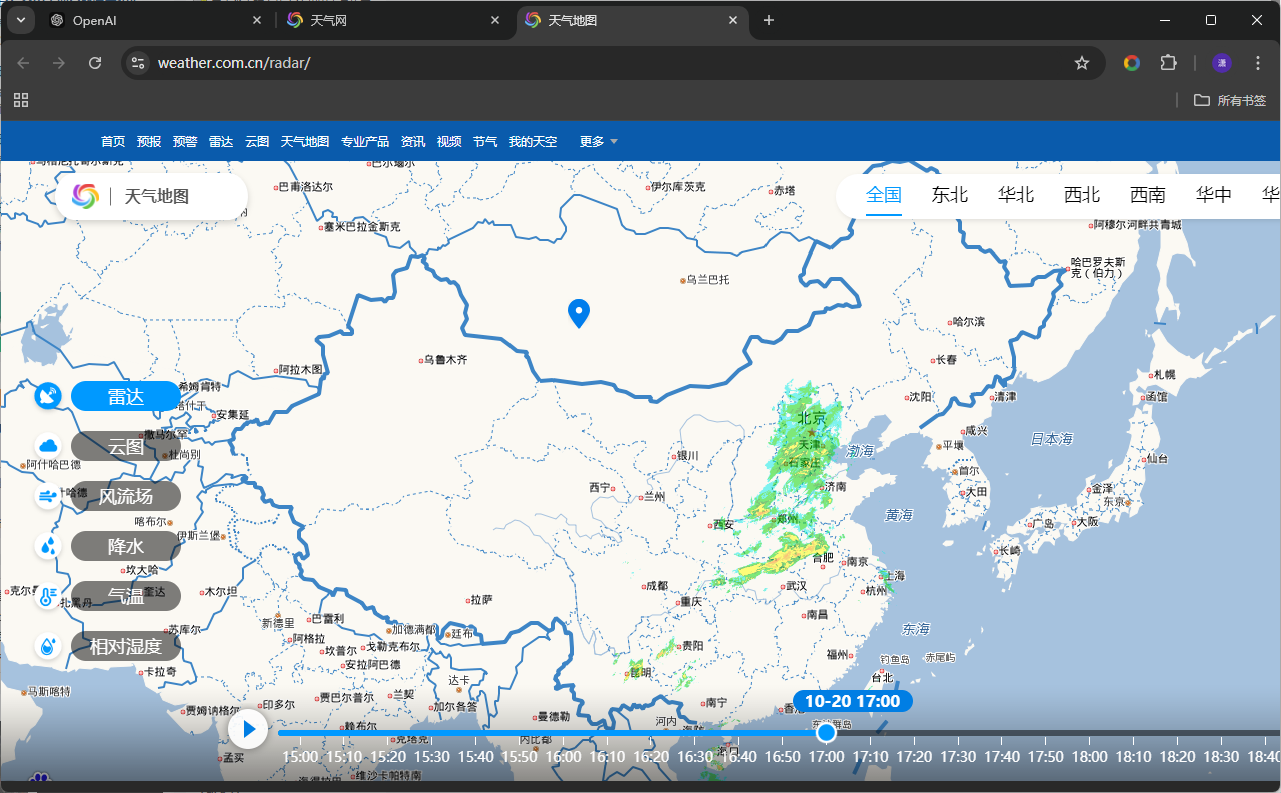
\includegraphics[width=\textwidth]{figures/weathermap.png}
    \caption{天气地图}\label{weathermap}
\end{figure}

\begin{figure}[!htbp]
    \centering
    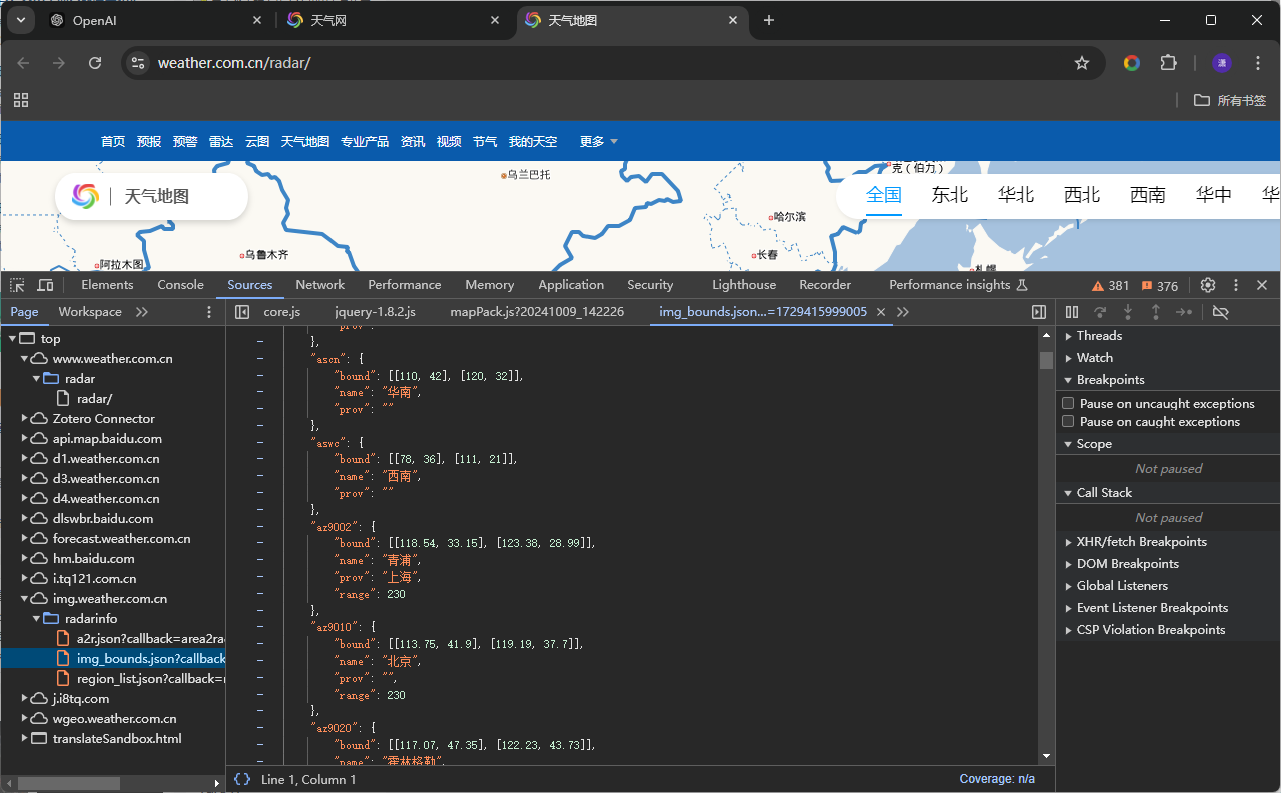
\includegraphics[width=\textwidth]{figures/image_bound_content.png}
    \caption{img\_bound请求回复报文体}\label{imgboundcontent}
\end{figure}

\begin{figure}[!htbp]
    \centering
    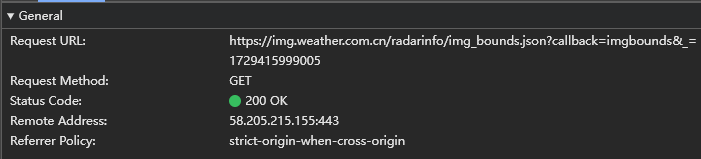
\includegraphics[width=\textwidth]{figures/image_bound_head.png}
    \caption{img\_bound请求报文头}\label{imgboundhead}
\end{figure}

\begin{figure}[!htbp]
    \centering
    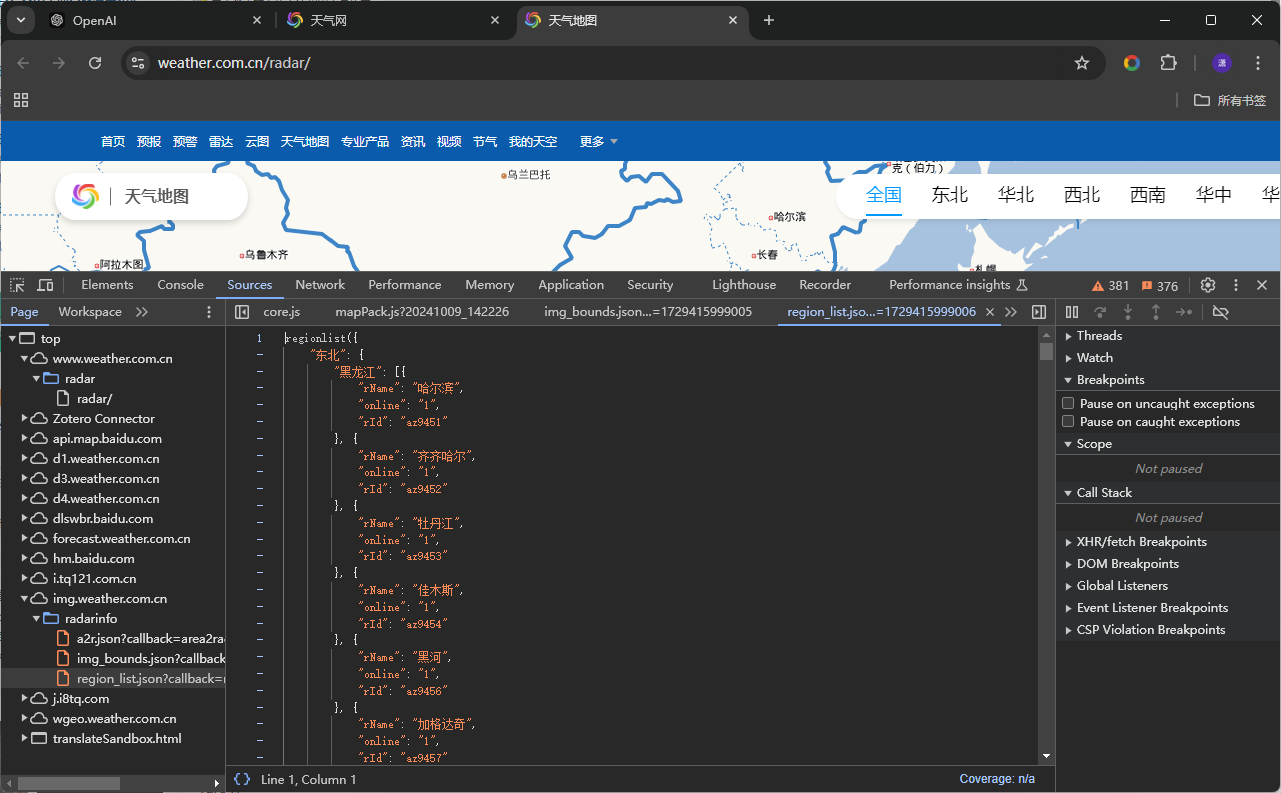
\includegraphics[width=\textwidth]{figures/region_list_content.png}
    \caption{region\_list请求回复报文体}\label{regionlistcontent}
\end{figure}

\begin{figure}[!htbp]
    \centering
    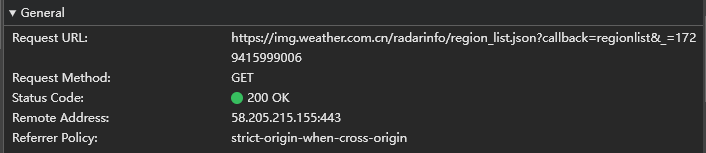
\includegraphics[width=\textwidth]{figures/region_list_head.png}
    \caption{region\_list请求报文头}\label{regionlisthead}
\end{figure}

\begin{figure}[!htbp]
    \centering
    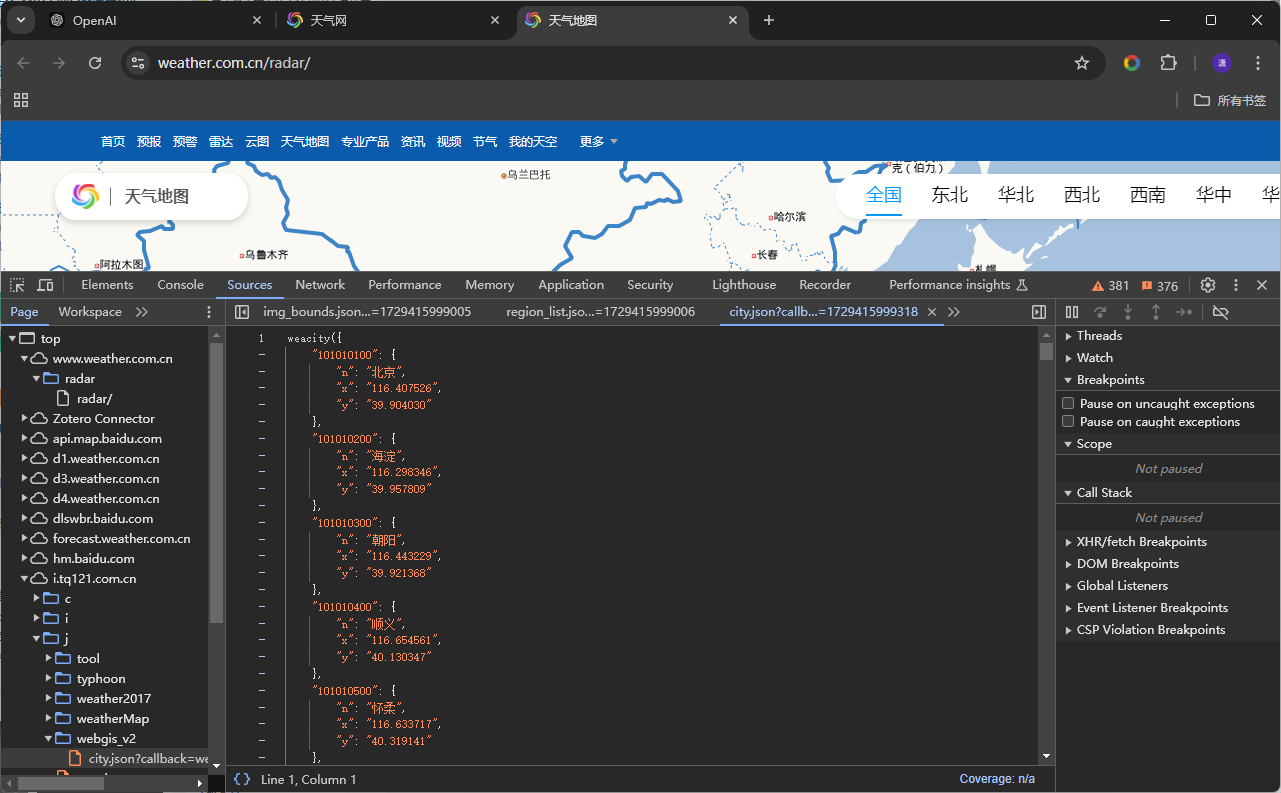
\includegraphics[width=\textwidth]{figures/city_js_content.png}
    \caption{city请求回复报文体}\label{cityjscontent}
\end{figure}

\begin{figure}[!htbp]
    \centering
    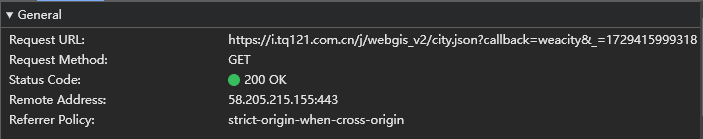
\includegraphics[width=\textwidth]{figures/city_js_head.png}
    \caption{city请求头}\label{cityjshead}
\end{figure}


\begin{figure}[!htbp]
    \centering
    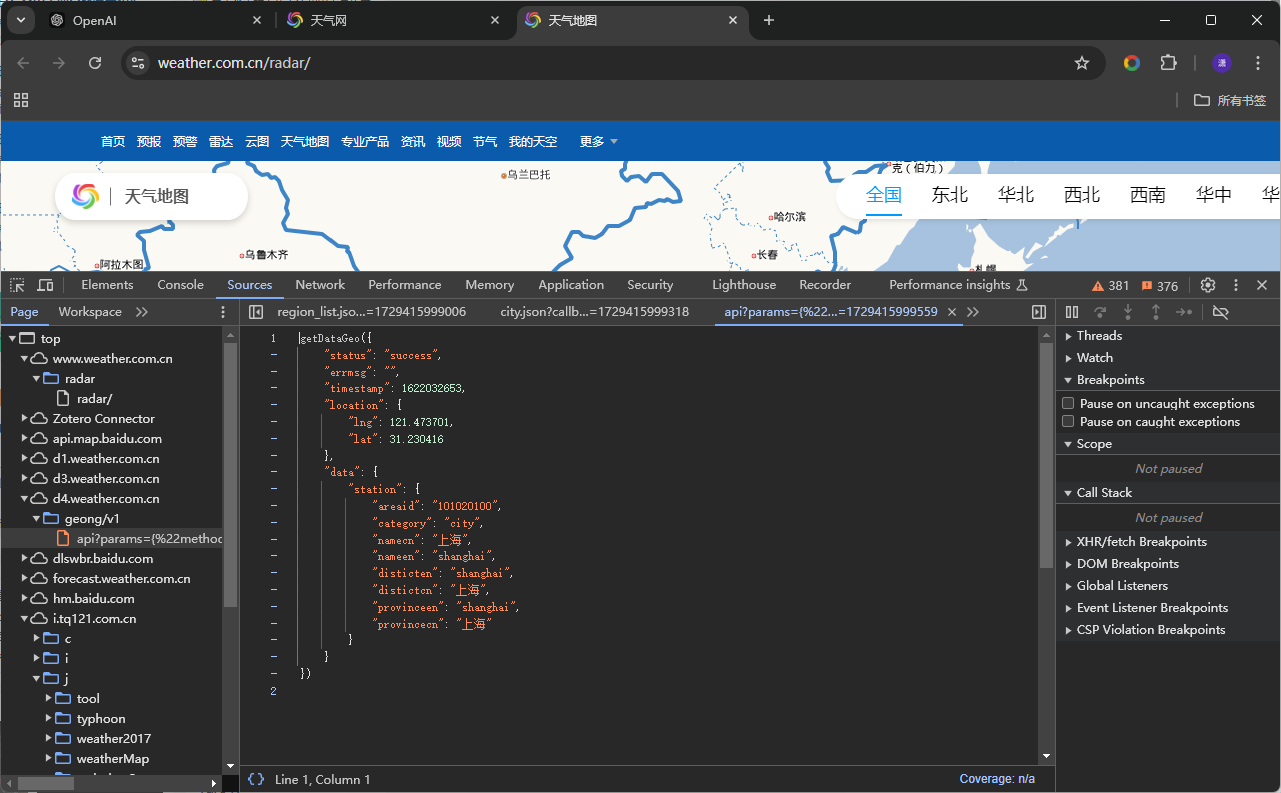
\includegraphics[width=\textwidth]{figures/city_info_content.png}
    \caption{api请求回复报文体}\label{cityinfocontent}
\end{figure}

\begin{figure}[!htbp]
    \centering
    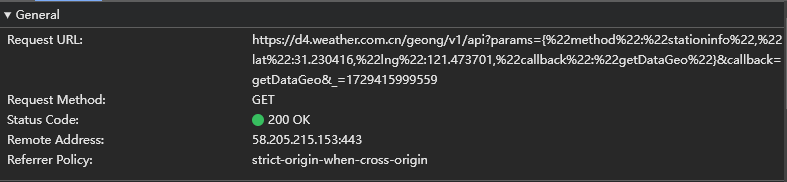
\includegraphics[width=\textwidth]{figures/city_info_head.png}
    \caption{api请求报文头}\label{cityinfohead}
\end{figure}

\begin{figure}[!htbp]
    \centering
    
\includegraphics[width=\textwidth]{figures/city_info_load.png}
    \caption{api请求载荷}\label{cityinfoload}
\end{figure}

\begin{figure}[!htbp]
    \centering
    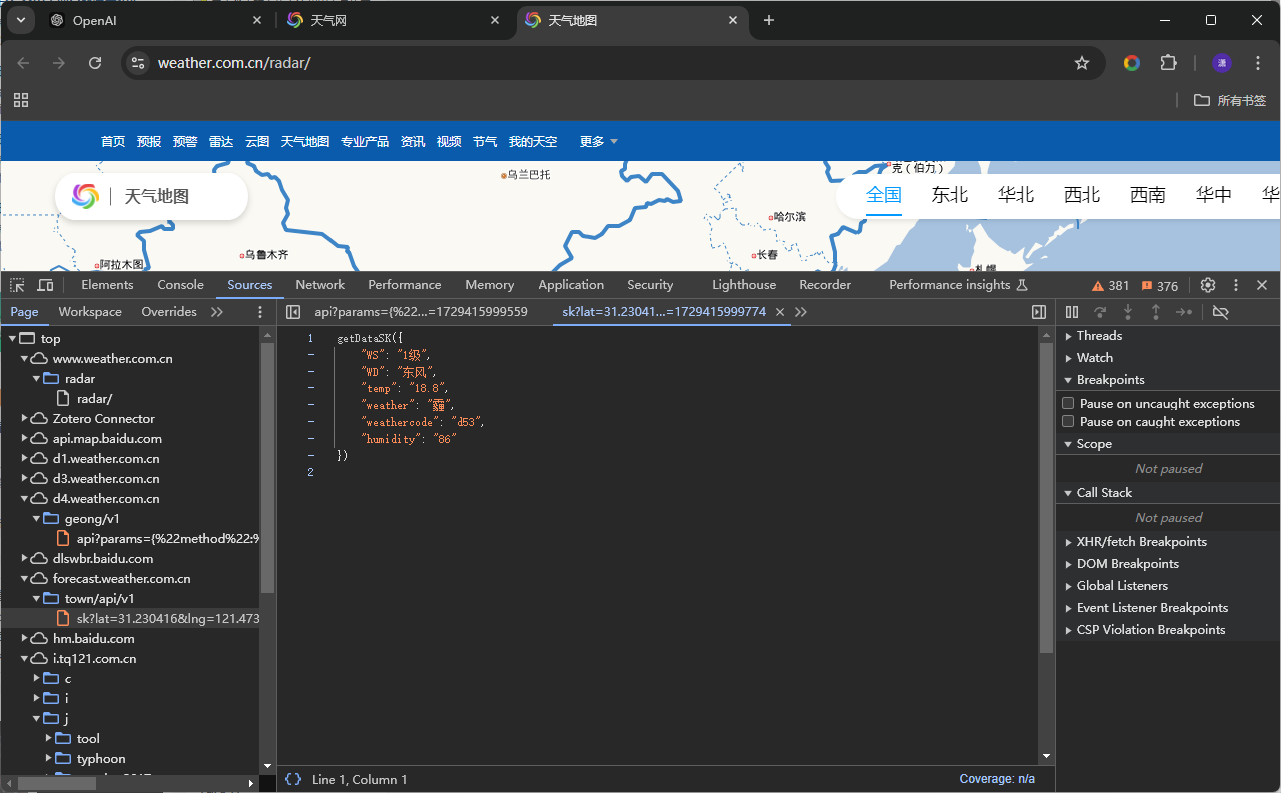
\includegraphics[width=\textwidth]{figures/weather_info_content.png}
    \caption{sk请求恢复报文体}\label{weatherinfocontent}
\end{figure}

\begin{figure}[!htbp]
    \centering
    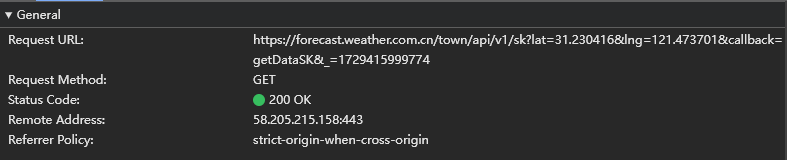
\includegraphics[width=\textwidth]{figures/weather_info_head.png}
    \caption{sk请求报文头}\label{weatherinfohead}
\end{figure}

\begin{figure}[!htbp]
    \centering
    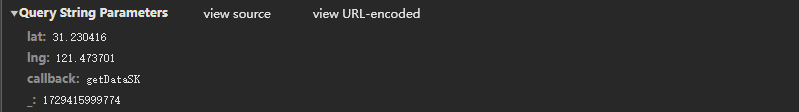
\includegraphics[width=\textwidth]{figures/weather_info_load.png}
    \caption{sk请求载荷}\label{weatherinfoload}
\end{figure}

